\section{Method}

\begin{figure*}[tb]
\centering
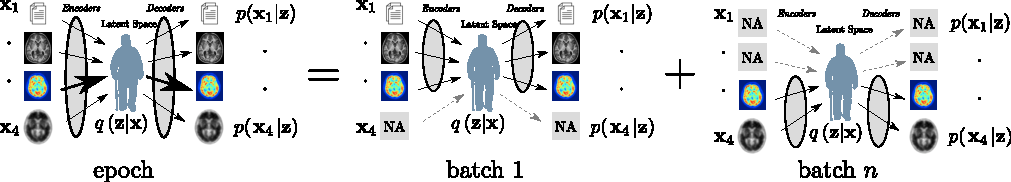
\includegraphics[width=\textwidth]{./tex/fig/model.pdf}
\caption{
Multi-view learning scheme in the presence of missing not available (NA) data.
Arrows represent trainable functions used as network encoders and decoders.
The contribution of datapoints to the model learning is reduced in.
}
\label{fig:model}
\end{figure*}

\begin{algorithm} % enter the algorithm environment
\caption{Model parameters optimization} % give the algorithm a caption
\label{alg:optim} % and a label for \ref{} commands later in the document
\begin{algorithmic} % enter the algorithmic environment
	\Require Initialize the model parameters $\phib, \thetab$. Set the optimizer learning rate.
	\While{$\phib, \thetab$ not converged}
		\State $\lb \leftarrow 0$
		\For{every dataset $d \in D$}
			\For{every datapoint $n \in N_d$}
				\For{every \textit{decoding} view $v \in V_{d,n}$}
					\State $\lb_v \leftarrow 0$
					\For{every \textit{encoding} view $w \in V_{d,n}$}
						\State Accumulate the cost of decoding $\xdnv$ through the encoder $q_{d,n,w}(\z)$:
						\State $\lb_v \leftarrow \lb_v + \EE{q_{d,n,w}(\z)}{\ln \p{\xdnv|\z, \thetab_v}} - \KL{q_{d,n,w}(\z)}{\pz}$.
					\EndFor
					\State Average the decoding cost and accumulate it in the total cost $\lb$:
					\State $\lb \leftarrow \lb + \frac{1}{V_{d,n}} \lb_v$.
				\EndFor
			\EndFor
		\EndFor
		\State $\thetab, \phib = \optim(\phib, \thetab, \nabla_{\phib} \lb, \nabla_{\thetab} \lb)$. \textit{Adam} optimizer used to maximie $\lb$.
	\EndWhile
\end{algorithmic}
\end{algorithm}
% \begin{algorithm} % enter the algorithm environment
% \caption{Calculate $y = x^n$} % give the algorithm a caption
% \label{alg1} % and a label for \ref{} commands later in the document
% \begin{algorithmic} % enter the algorithmic environment
%     \REQUIRE $n \geq 0 \vee x \neq 0$
%     \ENSURE $y = x^n$
%     \STATE $y \Leftarrow 1$
%     \IF{$n < 0$}
%         \STATE $X \Leftarrow 1 / x$
%         \STATE $N \Leftarrow -n$
%     \ELSE
%         \STATE $X \Leftarrow x$
%         \STATE $N \Leftarrow n$
%     \ENDIF
%     \WHILE{$N \neq 0$}
%         \IF{$N$ is even}
%             \STATE $X \Leftarrow X \times X$
%             \STATE $N \Leftarrow N / 2$
%         \ELSE[$N$ is odd]
%             \STATE $y \Leftarrow y \times X$
%             \STATE $N \Leftarrow N - 1$
%         \ENDIF
%     \ENDWHILE
% \end{algorithmic}
% \end{algorithm}


Let $\Dcal = \set{D_d}_{d=1}^D$ be a collection of $D$ independent datasets, where each dataset $D_d = \set{\xdn}_{n=1}^{N_d}$ is composed by $N_d$ independent data-points (\eg subjects in the case of medical imaging datasets).
To every dataset $D_d$ we associate a total number of $V_d$ available views
(\eg sets of clinical scores, imaging derived phenotypes extracted from multiple imaging modalities, \ldots),
and we assume that each data-point $\xdn = \set{\xdnv}_{v=1}^{V_{d,n}}$ is composed by $V_{d,n}$ views,
where $V_{d,n} \leq V_d$.
With the latest inequality we account for data-points with an arbitrary number of missing views.

For each view $\xdnv$ we propose the following generative latent variable model:
\begin{equation}\label{eq:model}
\begin{aligned}
&\z_{d,n} \sim \p{\z}, \\  % = \GaussStdDim{l} \\
&\xdnv \sim \p{\xdnv|\z_{d,n},\thetab_v},  % = \Gauss{\mub_c(\z)}{\Sigmab_c(\z) | \thetab_c}
\qquad \textnormal {for} \; v \; \textnormal{in} \; 1 \ldots V_{d,n} \leq V_d,
\end{aligned}
\end{equation}
where $\pz$ is a prior distribution for the latent variable $\z_{d,n}$ commonly shared by the $V_{d,n}$ views, and
where the likelihood functions $\p{\xdnv|\z_{d,n},\thetab_v}$ belong to a family of distributions parametrized by $\thetab_v$, which represents the view-specific generative parameters shared among all datasets.

The exact solution to the inference problem is given by the posterior $\p{\z|\set{\xdnv,\thetab_v}_{v=1}^{V_{d,n}}}$, that is not always computable analytically.
We can nevertheless look for its approximation $\qz$ through the \textit{Variational Inference} framework \citep{Blei2017}.
By introducing the latent variational approximation $\qz$, we can derive the following lower bound on the marginal log-likelihood for our generative model as follows:
\begin{equation}\label{eq:LB}
\begin{aligned}
\ln \p{\xdnv|\thetab_v} &= \ln \int \p{\xdnv|\z, \thetab_v} \p{\z} \; d\z \\
                        &= \ln \EE{\qz}{\frac{\p{\xdnv|\z, \thetab_v} \p{\z}}{\qz}} \\
                        &\geq \EE{\qz}{\ln \p{\xdnv|\z, \thetab_v}} - \KL{\qz}{\pz},
\end{aligned}
\end{equation}
where we compute the expectation with respect to an arbitrary distribution $\qz$.
To derive the last line of \eqnref{eq:LB} we leverage on the \textit{Jensen's inequality} applied to the logarithm function, and collect the result into a new expectation term and in the Kullback-Leibler divergence term ($\kl$).

With the right choice of the functional form of $\qz$, $\pz$, and $\p{\xdnv|\z, \thetab_v}$, the \rhs\ of \eqnref{eq:LB} becomes amenable to computation and maximization, yielding to the maximization of the \lhs, also known as the model evidence.

The common choice for the prior distribution $\pz$ is the multivariate isotropic Gaussian distribution $\Gausstd$,
while the choice for the likelihood function $\p{\xdnv|\z, \thetab_v}$ depends on the nature of the view $\xdnv$.
For example it can be parametrized as a multivariate Gaussian in the case of continuous data (\ie imaging derived phenotypes), as a Bernoulli likelihood for dichotomic data, as a Categorical likelihood for categorical data, \textit{etc}.
We define the distribution function $\qz$ to depend on a specific dataset $d$, data-point $n$, and view $w$, such that:
\begin{equation}\label{eq:q}
\begin{aligned}
\qz = q_{d,n,w}(\z) = \q{\z|\x_{d,n,w}, \phib_w},
\end{aligned}
\end{equation}
where $\phib_w$ represents the view-specific variational parameters shared among all datasets.
To force a link among views, we impose the inequality \eqnref{eq:LB} to hold for any $w$ in $1 \ldots V_{d,n}$.
We can hence average the right and left hand sides of \eqnref{eq:LB} across the $V_{d,n}$ views to give the lower bound:
\begin{equation}\label{eq:newLB}
\begin{aligned}
% \ln \p{\xdnv|\thetab_v} &\geq \underbrace{\frac{1}{V_{d,n}} \sum_{w=1}^{V_{d,n}}
%   \EE{q_{d,n,w}(\z)}{\ln \p{\xdnv|\z, \thetab_v}}
% - \KL{q_{d,n,w}(\z)}{\pz}}_{\LBn}. \\
\ln \p{\xdnv|\thetab_v} \geq \LBdnv = \frac{1}{V_{d,n}} \sum_{w=1}^{V_{d,n}} \LBdnvw,
\end{aligned}
\end{equation}
where
\begin{equation}\label{eq:LBdnvw}
\begin{aligned}
\LBdnvw = \EE{q_{d,n,w}(\z)}{\ln \p{\xdnv|\z, \thetab_v}} - \KL{q_{d,n,w}(\z)}{\pz}
\end{aligned}
\end{equation}
is the lower bound associated to the data-point $\xdn$ when its view $v$ is predicted from its view $w$.
Assuming independent observations, the marginal log-likelihood in the left hand side of \eqnref{eq:newLB} con be summed up over all the datasets, data-points, and views.
As a consequence, inference on the model generative parameters $\thetab = \set{\thetab_v}$ and variational parameters $\phib = \set{\phib_w}$ can be achieved by solving the maximization problem:
\begin{equation}\label{eq:argmax}
\begin{aligned}
\hat{\thetab}, \hat{\phib} &= \underset{\thetab, \phib}{\argmax} \sum_{d,n,v} \LBdnv \\
                           &= \underset{\thetab, \phib}{\argmax} \sum_{d,n,v} \frac{1}{V_{d,n}} \sum_{w=1}^{V_{d,n}} \LBdnvw.
\end{aligned}
\end{equation}
We use Algorithm \ref{alg:optim} to solve \eqnref{eq:argmax}.
The summation in \eqnref{eq:argmax} is done for every dataset $d$ along all the available data-points $n$ and their specific views $v$, although batching data-points with common views can speed up the computation by reducing the number of second level \textit{for} loop iterations in Algorithm \ref{alg:optim}.
If missing, a particular view $v$ will be simply not accounted for that specific observation, without having to discard all the other views that can still contribute to optimize \eqnref{eq:argmax}.
The presence of at least one common view among datasets acts as a link and allows the information to flow through all the datasets to the other views.

We observe that this model extends the Multi-Channel VAE \cite{Antelmi2019}, which is a multi-view extension of the VAE \cite{Kingma2013,Rezende2014}.
The authors of \cite{Antelmi2019} propose a multi-view generative model where they require all the observation in the training set to have all the available views, hence limited to model one dataset at a time (in the case of datasets with different views), after having discarded incomplete observations in that dataset.
We address this limitation by allowing missing views in the training set for some observations.
Similarly to \cite{Antelmi2019}, the trained model can estimate missing views from the available ones through the formula:
\begin{equation}\label{eq:reconstruction}
\begin{aligned}
\hat\xb_{d,n,v} = \frac{1}{V_{d, n}-1} \sum_{w=1, \,w\neq v}^{V_{d, n}} \EE{q_{d,n,w}(\z)}{\p{\xdnv|\z, \thetab_v}}.
\end{aligned}
\end{equation}

